\documentclass[a4paper,12pt]{article} 
\usepackage[utf8]{inputenc} % Acentos válidos sin problemas
\usepackage[spanish]{babel} % Idioma


\usepackage[backend=biber, style=alphabetic, sorting=ynt]{biblatex}
\bibliography{bibliografia.bib}
\nocite{*} % Añade todas las referencias de bib sin cita

%-----------------------------------INICIO DE PACKETES-------------------/
%-----------------------------------------------------------------------/
\usepackage{amsmath}   % Matemáticas: Comandos extras(cajas ecuaciones) |
\usepackage{amsthm}
\usepackage{amssymb}   % Matemáticas: Símbolos matemáticos              |
\usepackage{datetime}  % Agregar fechas                                 |
\usepackage{graphicx}  % Insertar Imágenes                              |
%\usepackage{biblatex} % Bibliografía                                   |
\usepackage{multicol}  % Creación de tablas                             |
\usepackage{longtable} % Tablas más largas                              |
\usepackage{xcolor}    % Permite cambiar colores del texto              |
\usepackage{tcolorbox} % Cajas de color                                 |
\usepackage{setspace}  % Usar espacios                                  |
\usepackage{fancyhdr}  % Para agregar encabezado y pie de página        |
\usepackage{lastpage}  %                                                 |
\usepackage{float}     % Flotantes                                      |
\usepackage{soul}      % "Efectos" en palabras                          |
\usepackage{hyperref}  % Para usar hipervínculos                        |
\usepackage{caption}   % Utilizar las referencias                       |
\usepackage{subcaption} % Poder usar subfiguras                         |
\usepackage{multirow}  % Nos permite modificar tablas                   |
\usepackage{array}     % Permite utilizar los valores para multicolumn  |
\usepackage{booktabs}  % Permite modificar tablas                       |
\usepackage{diagbox}   % Diagonales para las tablas                     |
\usepackage{colortbl}  % Color para tablas                              |
\usepackage{listings}  % Escribir código                               |
\usepackage{mathtools} % SIMBOLO :=                                     |
\usepackage{enumitem}  % Modificar items de Listas                      |
\usepackage{tikz}      %                                                |
\usepackage{lipsum}    % for auto generating text                       |
\usepackage{afterpage} % for "\afterpage"s                              |
\usepackage{pagecolor} % With option pagecolor={somecolor or none}|     |
\usepackage{xpatch}    % Color de lineas C & F
%\usepackage{glossaries} %                                              |
\usepackage{lastpage}    %                                              |   
\usepackage{csquotes}    %                                              |
%-----------------------------------------------------------------------\
%-----------------------------------FIN--- DE PACKETES-------------------\

\usepackage{pgfplots}     %                                             |
\pgfplotsset{compat=1.18} %           
\usepackage{etoolbox}
\usepackage{tikz,times}
\usepackage{verbatim}
\usetikzlibrary{mindmap,trees,backgrounds}
%--------------------------------/
%-------------------------------/
\usepackage[                 %   |
  headheight=15pt,  %            |
  letterpaper,  % Tipo de pag.   |
  left =1.5cm,  %  < 1 >         |
  right =1.5cm, %  < 1 >         | MARGENES DE LA PAGINA
  top =2cm,     %  < 1.5 >       |
  bottom =1.5cm %  < 1.5 >       |
]{geometry}     %                |
%-------------------------------\
%--------------------------------\

%----------------------------------------------------------------------/
%-------------------Encabezado y Pie de Pagina-----------------------/ |
%--------------------------------------------------------------------\ |
%\fancyhf{}
%\pagestyle{fancy}

\fancypagestyle{firstpage}{  
    \fancyhead[L]{}
    \fancyhead[R]{}     
    \fancyfoot[L]{}
    \fancyfoot[C]{}
    \fancyfoot[R]{\thepage\ de \pageref*{LastPage}}    
    \renewcommand{\headrulewidth}{0pt} 
    \xpretocmd\headrule{}{}{\PatchFailed}
}

\fancypagestyle{fancy}{  
    \fancyhead[L]{\textbf{Semestre: 2024-2}}
    \fancyhead[C]{}     
    \fancyhead[R]{}     

    \fancyfoot[L]{\texttt{Skynet Scribes}}
    \fancyfoot[C]{\texttt{IA}}
    \fancyfoot[R]{\thepage\ de \pageref*{LastPage}}

    \renewcommand{\headrulewidth}{1pt} 
    \xpretocmd\headrule{}{}{\PatchFailed}
    \renewcommand{\footrulewidth}{1.5pt} 
    \xpretocmd\footrule{}{}{\PatchFailed}
}

\fancypagestyle{fancyref}{  
    \fancyhead[L]{}
    \fancyhead[R]{}     
    \fancyfoot[L]{\texttt{Skynet Scribes}}
    \fancyfoot[C]{\texttt{IA}}
    \fancyfoot[R]{\thepage\ de \pageref*{LastPage}}    
    \renewcommand{\headrulewidth}{0pt} 
    \xpretocmd\headrule{}{}{\PatchFailed}
}
%--------------------------------------------------------------------\ |
%-------------------Encabezado y Pie de Pagina-----------------------/ |
%------------------------------------------------------------FIN----/


%--------------------------------------------------------------------/
%------------------- LISTA DE COLORES ------------------------------/ 
\definecolor{ProcessBlue}{RGB}{0,176,240}
\definecolor{NavyBlue}{RGB}{0,110,184}
\definecolor{Cyan}{RGB}{0,174,239}
\definecolor{MidnightBlue}{RGB}{0,103,49}
\definecolor{ForestGreen}{RGB}{0,155,85}
\definecolor{Goldenrod}{RGB}{255,223,66}
\definecolor{YellowGreen}{RGB}{152,204,112}
\definecolor{Sepia}{RGB}{103,24,0}
\definecolor{Peach}{RGB}{247,150,90}
\definecolor{CarnationPink}{RGB}{242,130,180}
\definecolor{Fuchsia}{RGB}{140,54,140}
\definecolor{WildStrawberry}{RGB}{238,41,103}
\definecolor{blueRY}{RGB}{13,164,245}

\definecolor{Grass}{RGB}{41,238,53}
\definecolor{Meadow}{RGB}{6,243,67}
\definecolor{jellyfish}{RGB}{109,14,130}
\definecolor{rubber}{RGB}{229,27,232}
\definecolor{bullet}{RGB}{225,31,90}
\definecolor{midnight}{RGB}{31,90,225}
\definecolor{sun}{RGB}{241,152,7}
\definecolor{water}{RGB}{16,229,183}

%------------------- COLORES CÓDIGO ---------------------- |
%------------------- COLORES JAVA ---------------------- |
\definecolor{backcolour}{RGB}{6,6,6} 
%\definecolor{backcolour}{RGB}{181,181,181} 
\definecolor{codeclassjava}{RGB}{246,113,59}
\definecolor{codegreen}{RGB}{17,225,48}
\definecolor{codenumizq}{RGB}{17,17,17}
\definecolor{codestringjava}{RGB}{51,240,234}
\definecolor{codesymboljava}{RGB}{255,5,0} 
\definecolor{yellowpoint}{RGB}{244,235,100} 
%------------------- COLORES JAVA ---------------------- |
%------------------- COLORES PYTHON -------------------- |
\definecolor{backcolourPY}{RGB}{6,6,6} 
%\definecolor{backcolour}{RGB}{181,181,181} 
\definecolor{codegreenPY}{RGB}{17,225,48}
\definecolor{codeclassPY}{RGB}{246,113,59}
\definecolor{codenumizq}{RGB}{17,17,17}
\definecolor{codestringPY}{RGB}{90,128,220}
\definecolor{codesymboljava}{RGB}{255,5,0} 
%------------------- COLORES PYTHON -------------------- |
%------------------- COLORES TERMINAL-------------------- |
\definecolor{backcolourTerminal}{rgb}{0.0, 0.0, 0.0} % Negro
\definecolor{codeclassTerminal}{rgb}{1.0, 1.0, 1.0} % Blanco
\definecolor{codestringTerminal}{rgb}{0.0, 0.6, 0.0} % Verde
\definecolor{codecommentTerminal}{rgb}{0.5, 0.5, 0.5} % Gris
\definecolor{codenumizqTerminal}{rgb}{0.0, 0.0, 1.0} % Azul
\definecolor{codeoptionTerminal}{rgb}{0.4, 0.4, 1.0} % Azul claro para opciones
\definecolor{yellowTerminal}{RGB}{238,200,62}
%------------------- COLORES TERMINAL-------------------- |
%------------------- COLORES CÓDIGO ---------------------- |



%------------------- LISTA DE COLORES -------------------------------\
%---------------------------------------------------------------------\

%-------------- ESTILO de Código PYTHON -----------------------------|
\lstdefinestyle{mystylepython}{
    backgroundcolor=\color{backcolourPY},
    commentstyle=\color{codecommentTerminal},
    keywordstyle=\color{blueRY},
    numberstyle=\tiny\color{codenumizq},
    stringstyle=\color{codestringPY},
    basicstyle=\footnotesize\ttfamily\color{white},
    breakatwhitespace=false,
    breaklines=true,
    captionpos=b,
    keepspaces=true,
    numbers=left,
    numbersep=5pt,
    showspaces=false,
    showstringspaces=false,
    showtabs=false,
    tabsize=2,
    escapechar=\&,
    literate=                
        {;}{{\textcolor{yellowpoint}{;}}}1
        {+}{{\textcolor{yellowpoint}{+}}}1
        {-}{{\textcolor{yellowpoint}{-}}}1
        {\{}{{\textcolor{yellowpoint}{\{}}}1
        {\}}{{\textcolor{yellowpoint}{\}}}}1
        {[}{{\textcolor{yellowpoint}{[}}}1
        {]}{{\textcolor{yellowpoint}{]}}}1
        {=}{{\textcolor{yellowpoint}{=}}}1
        {:}{{\textcolor{yellowpoint}{:}}}1
        {<}{{\textcolor{yellowpoint}{<}}}1
        {>}{{\textcolor{yellowpoint}{>}}}1
}
%-------------- ESTILO de Código PYTHON -----------------------------|
%-------------- ESTILO de Código TERMINAL ---------------------------|
\lstdefinestyle{mystyleTerminal}{
    backgroundcolor=\color{backcolourTerminal},
    commentstyle=\color{codecommentTerminal},
    keywordstyle=\color{codeclassTerminal},
    numberstyle=\tiny\color{backcolourTerminal},
    stringstyle=\color{codestringTerminal},
    basicstyle=\footnotesize\ttfamily\color{codeclassTerminal},
    breakatwhitespace=false,
    breaklines=true,
    captionpos=b,
    keepspaces=true,
    numbers=left,
    numbersep=5pt,
    showspaces=false,
    showstringspaces=false,
    showtabs=false,
    tabsize=4,    
    escapechar=\&,
    literate = 
            {--}{{\textcolor{codecommentTerminal}{--}}}2            
}
% Usar el estilo de código
\lstset{style=mystyleTerminal}
%-------------- ESTILO de Código TERMINAL ---------------------------|
\pagestyle{fancy}

\usepackage{algpseudocode}

\begin{document}%----------------------INICIO DOCUMENTO------------|
%------------------------------------------------------------------|
\begin{titlepage}
\center 
\newcommand{\HRule}{\rule{\linewidth}{0.5mm}} 

%---------------------
%	ESCUDO
%---------------------

\includegraphics[width=4.5cm]{IMA/cienciasWhite.png}

%----------------------------
%	TITULO
%----------------------------
\quad \\[0.2cm]
\textsc{\huge Facultad de Ciencias}\\[.6cm] 
\textsc{\huge Inteligencia Artificial}\\[0.5cm]

%-------------
%	TRABAJO
%-------------
\makeatletter
    \HRule \\ [0.4cm]
        { \huge \bfseries Exploradores de laberinto}\\
    \HRule \\ [0.4cm]
    
\vspace{2mm}

%----------------------------
%	Nombre del Equipo
%----------------------------
\begin{flushleft}
    \Large{Equipo:} \texttt{\Large Skynet Scribes}
\end{flushleft}
%----------------------------
%	Número de practica
%----------------------------
\begin{flushleft}
    \Large{Número de practica:} \texttt{\Large 02}\\[0.8cm]
\end{flushleft}


%-------------------
%	AUTORES
%-------------------
\begin{minipage}{0.8\textwidth}
    \begin{flushright}
        \textbf{\large{Carlos Daniel Cortés Jiménez}}\\    
        420004846        
    \end{flushright}
\end{minipage}

\vspace{5mm}

\begin{minipage}{0.4\textwidth}
        \textbf{\large{Sarah Sophía Olivares García}}\\
        318360638
\end{minipage}
\begin{minipage}{0.4\textwidth}
    \begin{flushright}
        \textbf{\large{Marco Silva Huerta}}\\
        316205326        
    \end{flushright}
\end{minipage}

\vspace{5mm}

\begin{minipage}{0.4\textwidth}
        \textbf{\large{Juan Daniel Barrera Holan}}\\    
        417079372
\end{minipage}
\begin{minipage}{0.4\textwidth}
    \begin{flushright}
        \textbf{\large{Laura Itzel Tinoco Miguel}}\\
        316020189
    \end{flushright}
\end{minipage}

\vspace{10mm}
%-------------------
%	PROFESORES
%-------------------

\begin{minipage}{0.8\textwidth}
    \begin{flushleft} \large
        Profesora: Cecilia Reyes Peña\\
        Ayudante teoría: Karem Ramos Calpulalpan \\
        Ayudante laboratorio: Tania Michelle Rubí Rojas\\                    
    \end{flushleft}
\end{minipage}

\vspace{20mm}

\begin{minipage}{0.4\textwidth}
    %---------------
    %	S E M E S T R E
    %---------------
    \textcolor{white}{Semestre}\\
    \large\textbf{Semestre 2024-2}      
\end{minipage}
\begin{minipage}{0.4\textwidth}
    %---------------
    %	F E C H A
    %---------------
    \begin{flushright}
        {\large Fecha de entrega:\\
         \textbf{28 de Febrero del 2024}}
    \end{flushright}
\end{minipage}

\makeatother

\vfill 
\end{titlepage}

\newpage

%% Investigación sobre las dos preguntas
%%  comparando los algoritmos de búsqueda
\section{Algoritmo $A^{*}$}

% --------------------------------------------------------------\
% -------------------------------------------------------------\
\subsection*{Introducción}
% -------------------------------------------------------------\
% --------------------------------------------------------------\

El algoritmo $A^{*}$, concebido en 1968 por Peter Hart, Nils Nilsson, y Bertram Raphael, se erige como 
un pilar en la búsqueda de caminos dentro del vasto dominio de la inteligencia artificial. Este 
algoritmo trasciende la simpleza de métodos tradicionales, como la Búsqueda en Anchura (BFS) y la 
Búsqueda en Profundidad (DFS), mediante la incorporación de una función heurística. Esta heurística 
orienta la exploración hacia el objetivo de manera eficiente, optimizando el trayecto en términos de 
coste y distancia. Su versatilidad le permite adaptarse a una amplia gama de aplicaciones, desde la 
conducción autónoma y la robótica hasta la generación de rutas en videojuegos y aplicaciones de mapeo 
geográfico.

% --------------------------------------------------------------\
% -------------------------------------------------------------\
\subsection*{¿Cómo funciona?}
% -------------------------------------------------------------\
% --------------------------------------------------------------\




% --------------------------------------------------------------\
% -------------------------------------------------------------\
\subsection*{Algoritmo $A^{*}$ vs BFS}
% -------------------------------------------------------------\
% --------------------------------------------------------------\

A diferencia de la Búsqueda en Anchura (BFS), que adopta un enfoque no ponderado y equitativo en su 
exploración expandiendo todos los nodos vecinos con igual prioridad, el algoritmo $A^{*}$ introduce 
una estrategia de búsqueda ponderada. Esta estrategia se centra en minimizar una función de coste 
\(f(n) = g(n) + h(n)\), donde \(g(n)\) representa el coste exacto desde el nodo inicial hasta el nodo 
\(n\), y \(h(n)\) es la heurística que estima el coste mínimo desde \(n\) hasta el objetivo. Esta 
dualidad permite a $A^{*}$ explorar de forma selectiva aquellos caminos que parecen más prometedores, 
reduciendo significativamente el volumen de cálculo y garantizando la identificación del trayecto óptimo.

% --------------------------------------------------------------\
% -------------------------------------------------------------\
\subsection*{Ventajas}
% -------------------------------------------------------------\
% --------------------------------------------------------------\
\begin{itemize}
    \item \textbf{Optimalidad y Complejidad:} $A^{*}$ garantiza encontrar la ruta más corta hacia el 
                objetivo, siempre que la heurística empleada sea admisible y consistente. Esta 
                característica lo distingue como un algoritmo de búsqueda óptima.
    \item \textbf{Eficiencia:} Al priorizar nodos basándose en el coste total estimado \(f(n)\), $A^{*}$ 
                es capaz de descartar rutas menos prometedoras de manera precoz, agilizando la 
                consecución de su meta.
    \item \textbf{Flexibilidad Heurística:} La posibilidad de adaptar la heurística \(h(n)\) según 
                las particularidades del problema permite una optimización específica del 
                rendimiento de búsqueda.
\end{itemize}
% --------------------------------------------------------------\
% -------------------------------------------------------------\
\subsection*{Desventajas}
% -------------------------------------------------------------\
% --------------------------------------------------------------\
\begin{itemize}
    \item \textbf{Dependencia Heurística:} La eficacia del algoritmo está intrínsecamente ligada 
                a la calidad de la heurística \(h(n)\). Una heurística pobre puede resultar en 
                una exploración ineficiente y un mayor consumo de recursos.
    \item \textbf{Requerimientos de Memoria:} El mantenimiento de las listas abierta y cerrada,
                especialmente en espacios de búsqueda vastos, puede conducir a un elevado 
                consumo de memoria, superando en ocasiones a alternativas más simples como BFS.
\end{itemize}

% --------------------------------------------------------------\
% -------------------------------------------------------------\
\section{Distancia Manhattan}
% -------------------------------------------------------------\
% --------------------------------------------------------------\

La \textit{distancia de Manhattan} es una métrica que mide la distancia entre dos puntos en un espacio 
euclidiano multidimensional, y esta basada en líneas paralelas a los ejes de coordenadas en lugar de 
una línea recta, como puede ser un plano cartesiano, se emplea en inteligencia artificial y diversos 
campos (que incluyen la teoría de grafos, geometría computacional y optimización).\\ 


En el ámbito de la inteligencia artificial, se usa con frecuencia en algoritmos heurísticos como $A^{*}$ 
(A-estrella) para resolver problemas de búsqueda de caminos. El uso principal de esta medida es en 
situaciones donde el desplazamiento entre dos ubicaciones se limita a movimientos verticales u 
horizontales, como sucede en la planificación de rutas.\\ 


La razón por la que se llama \textit{Manhattan} a esta distancia es porque, en una cuadrícula de calles 
de ciudades como Manhattan, para ir de un punto a otro hay que moverse siguiendo las manzanas 
delimitadas por las calles horizontales y verticales en ángulos rectos. Entonces la distancia de 
\textit{Manhattan} es una medida básica en inteligencia artificial, especialmente para resolver 
problemas de búsqueda de rutas y planificación, gracias a su simpleza y eficacia en escenarios con 
movimientos restringidos a líneas rectas horizontales y verticales.\\ 


Planear rutas en entornos urbanos, especialmente en ciudades con calles ortogonales como Nueva York,
es un ejemplo de uso real de la distancia de Manhattan como heurística. Por ejemplo: Se puede usar 
en una app de mapas para hallar la ruta más corta desde donde estás hasta un punto específico en 
una ciudad con calles que se cruzan formando cuadras. \textit{distancia de Manhattan} puede servir 
como una guía para calcular la distancia que queda hasta llegar a tu destino.\\ 


O imagina que estás manejando en tu carro y tienes que ir desde un cruce $A$ hasta otro cruce $B$ 
en una ciudad con calles dispuestas en forma de cuadrícula. ¿Puedes determinar la 
\textit{distancia de Manhattan} entre $A$ y $B$ sumando el número de cuadras que necesitas recorrer 
en dirección horizontal y vertical para llegar de $A$ a $B$, sin considerar los obstáculos como 
edificios o restricciones de tráfico?\\ 


La distancia de Manhattan proporciona una estimación precisa del recorrido necesario en automóvil,
ya que las rutas siguen generalmente un patrón de calles y avenidas en ángulos rectos. A pesar de
que en la práctica puedan existir variaciones debido a las limitaciones del tráfico o la disposición
exacta de las calles, la distancia de Manhattan aún es una buena aproximación y puede ayudar a los 
sistemas de mapas para calcular rutas eficientes. \\ 

Así que, la distancia de Manhattan es empleada en aplicaciones de mapas y navegación como una 
heurística para estimar el tiempo y la distancia restante hasta un destino en entornos urbanos 
donde las calles siguen una disposición de cuadrícula ortogonal. Ayuda a los conductores a tomar 
decisiones informadas sobre sus rutas y permite que las aplicaciones de navegación calculen rutas 
óptimas de manera más eficiente.\\ 


La fórmula para calcular la distancia de Manhattan entre dos puntos $A(x_1, y_1)$ y $B(x_2,y_2)$,
en un espacio bidimensional es:
\begin{center}
    D = $|x_1 - x_2| + |y_1 - y_2|$
\end{center}

Donde $|x_1 - x_2|$ representa la diferencia en la coordenada x entre los dos puntos y  
$|y_1 - y_2|$ representa la diferencia en la coordenada y entre los dos puntos.\\ 


En pocas palabras la elección de la distancia Manhattan como heurística en la implementación de 
$A^{*}$ se fundamenta en su capacidad para estimar costes de manera coherente y admisible en entornos 
cuadriculados, donde los movimientos están restringidos a las direcciones cardinales. 
Esta simplicidad y eficacia la convierten en una heurística ideal para muchos escenarios de búsqueda 
en laberintos y grillas.

% --------------------------------------------------------------\
% -------------------------------------------------------------\
\subsection*{Pseudocódigo}
% --------------------------------------------------------------\
% -------------------------------------------------------------\

\begin{verbatim}
    función distancia_manhattan(nodo_actual, nodo_objetivo):
        diferencia_x = abs(nodo_actual.x - nodo_objetivo.x)
        diferencia_y = abs(nodo_actual.y - nodo_objetivo.y)
        return diferencia_x + diferencia_y
    \end{verbatim}

% -------------------------------------------------------------\
% --------------------------------------------------------------\
\section{Otras heurísticas}
% -------------------------------------------------------------\
% --------------------------------------------------------------\

Otros dos ejemplos de heurísticas que se pueden usar en el algoritmo $A^{*}$ son:

\begin{itemize}
    \item Distancia Euclidiana:
        Se utiliza como métrica para calcular la separación entre puntos en un espacio euclidiano, 
        ya sea en el plano o en el espacio tridimensional. Se utiliza el teorema de Pitágoras para 
        calcular la longitud del segmento de línea recta que une los dos puntos. La distancia 
        euclidiana es una heurística admisible, no obstante, puede no ser uniforme en todos los 
        casos, especialmente en ambientes con obstáculos donde la ruta más directa puede no ser 
        una línea recta.

        La fórmula para la distancia euclidiana entre dos puntos $A(x_1, y_1)$ y $B(x_2,y_2)$, 
        en un espacio bidimensional es:
        \begin{center}
            D = $\sqrt{(x_2 - x_1)^2 + (y_2 - y_1)^2}$
        \end{center}

    \item  Distancia de Chebyshev:
        \begin{itemize}
            \item La distancia de Chebyshev se usa como métrica para calcular la distancia entre 
                    dos puntos en un espacio de rejilla, donde el movimiento está permitido en todas 
                    las direcciones (horizontal, vertical y diagonal).
            \item La distancia de Chebyshev en entornos de rejilla es una heurística que cumple 
                    con la propiedad de consistencia, lo que la hace admisible.
            \item Estas reglas proporcionan estimaciones del costo restante para alcanzar el 
                    objetivo desde cualquier nodo dado en un grafo de búsqueda, lo que asiste 
                    al algoritmo $A^{*}$ a dirigir su búsqueda hacia el objetivo de forma más 
                    eficaz. Depende del problema específico y de las características del 
                    espacio de búsqueda la elección de la heurística.
        \end{itemize}
        
        La fórmula para la distancia euclidiana entre dos puntos $A(x_1, y_1)$ y $B(x_2,y_2)$, en un espacio bidimensional se calcula como la máxima de las diferencias absolutas en las coordenadas \textit{x} y \textit{y}
        \begin{center}
            D = $max(|x_2 - x_1|,|y_2 - y_1|)$
        \end{center}
\end{itemize}
%-------------------------------------------

%% Reporte final de la comparación 
%%  del código con la teoría
% --------------------------------------|
% -------------------------------------|
% ------------------------------------|
\section{Comparación de Resultados} 
% ------------------------------------\
% --------------------------------------\
% ----------------------------------------\
{\large\textbf{DFS:}}

\begin{enumerate}
    \item \textbf{Enfoque:} Backtracking, exploración profunda.
    \item \textbf{Exploración:} Se adentra tanto como sea posible antes de retroceder.
    \item \textbf{Optimización:} No garantiza encontrar la solución más corta.
    \item \textbf{Encuentra:} Una solución y muestra la ruta.
    \item \textbf{Distancia:} No considera la distancia, no hay garantía de que use la ruta más corta.
    \item \textbf{Eficiencia:} Puede ser eficiente en laberintos con caminos ramificados y no es 
    necesario encontrar la ruta más corta.
\end{enumerate}

\begin{figure}[h]
    \centering
    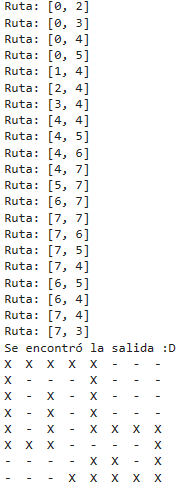
\includegraphics[scale = .6]{IMA/captuDFS.png}
    \caption{DFS}
    \label{fig:enter-label}
\end{figure}
\vspace{0.5cm}

{\large\textbf{BFS:}}

\begin{enumerate}
    \item \textbf{Enfoque:} Exploración nivel por nivel.
    \item \textbf{Exploración:} Comienza explorando todos los nodos a una 
    distancia \(d\) antes de pasar a los nodos a una distancia \(d+1\).
    \item \textbf{Optimización:} Garantiza encontrar la solución más corta. Garantiza la optimización.
    \item \textbf{Distancia:} Encuentra la ruta más corta desde el inicio hasta la salida.
    \item \textbf{Eficiencia:}Evita Explorar caminos no óptimos.
    \item \textbf{Evita:} Explorar caminos no óptimos.
\end{enumerate}

\begin{figure}[h]
    \centering
    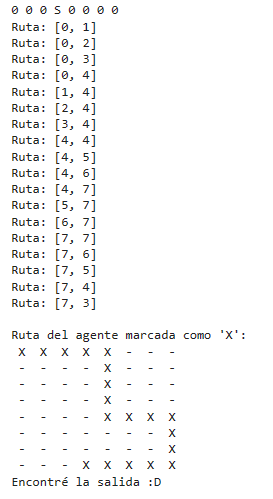
\includegraphics[scale = .6]{IMA/captuBFS.png}
    \caption{BFS}
    \label{fig:enter-label}
\end{figure}
\vspace{0.5cm}

\textbf{Ejemplo:}\\

Si elegimos el Laberinto 02, ambos algoritmos van a encontrar la salida. La diferencia sería:

\begin{itemize}
    \item \textbf{DFS:} Va a mostrar una ruta más larga pero válida.
    \item \textbf{BFS:} Va a garantizar la ruta más corta.
\end{itemize}

Entonces, la elección depende de nuestra prioridad, ya sea optimización o la exploración 
de diferentes caminos.
%-------------------------------------------

% ----------------------|
% Referencias           |
% Forma de Compilar     |
% pdflatex main.tex     |
% biber main            |
% pdflatex main.tex     |
\newpage %              |
\thispagestyle{fancyref}
\printbibliography %    |
% ----------------------|

\end{document}%----------------------F I N DOCUMENTO---------------|
%------------------------------------------------------------------|
